\documentclass[]{article}
\usepackage{lmodern}
\usepackage{amssymb,amsmath}
\usepackage{ifxetex,ifluatex}
\usepackage{fixltx2e} % provides \textsubscript
\ifnum 0\ifxetex 1\fi\ifluatex 1\fi=0 % if pdftex
  \usepackage[T1]{fontenc}
  \usepackage[utf8]{inputenc}
\else % if luatex or xelatex
  \ifxetex
    \usepackage{mathspec}
    \usepackage{xltxtra,xunicode}
  \else
    \usepackage{fontspec}
  \fi
  \defaultfontfeatures{Mapping=tex-text,Scale=MatchLowercase}
  \newcommand{\euro}{€}
\fi
% use upquote if available, for straight quotes in verbatim environments
\IfFileExists{upquote.sty}{\usepackage{upquote}}{}
% use microtype if available
\IfFileExists{microtype.sty}{%
\usepackage{microtype}
\UseMicrotypeSet[protrusion]{basicmath} % disable protrusion for tt fonts
}{}
\usepackage[margin=1in]{geometry}
\ifxetex
  \usepackage[setpagesize=false, % page size defined by xetex
              unicode=false, % unicode breaks when used with xetex
              xetex]{hyperref}
\else
  \usepackage[unicode=true]{hyperref}
\fi
\hypersetup{breaklinks=true,
            bookmarks=true,
            pdfauthor={Yago Durán Cid},
            pdftitle={Applied Logistic Regression - Exercise Week 4},
            colorlinks=true,
            citecolor=blue,
            urlcolor=blue,
            linkcolor=magenta,
            pdfborder={0 0 0}}
\urlstyle{same}  % don't use monospace font for urls
\setlength{\parindent}{0pt}
\setlength{\parskip}{6pt plus 2pt minus 1pt}
\setlength{\emergencystretch}{3em}  % prevent overfull lines
\setcounter{secnumdepth}{0}

%%% Use protect on footnotes to avoid problems with footnotes in titles
\let\rmarkdownfootnote\footnote%
\def\footnote{\protect\rmarkdownfootnote}

%%% Change title format to be more compact
\usepackage{titling}

% Create subtitle command for use in maketitle
\newcommand{\subtitle}[1]{
  \posttitle{
    \begin{center}\large#1\end{center}
    }
}

\setlength{\droptitle}{-2em}
  \title{Applied Logistic Regression - Exercise Week 4}
  \pretitle{\vspace{\droptitle}\centering\huge}
  \posttitle{\par}
  \author{Yago Durán Cid}
  \preauthor{\centering\large\emph}
  \postauthor{\par}
  \predate{\centering\large\emph}
  \postdate{\par}
  \date{06/06/2015}



\begin{document}

\maketitle


\textbf{WEEK 4}

\emph{Exercise 1:}

The data in hyponatremia.dta derive from an epidemiological study of
hyponatremia (a life-threatening condition) among runners of the 2002
Boston Marathon. Hyponatremia is defined as an electrolyte disturbance
in which the serum sodium concentration is lower than normal
(\textless{}135 mmol/l). The aim of the study was to determine whether a
runner experienced hyponatremia and to identify the principal risk
factors. Participants in the 2002 Boston Marathon completed a survey
including demographic and anthropometric characteristics (Body Mass
Index) one or two days before the race. After the race, runners provided
a blood sample in order to measure their serum sodium concentration and
completed a questionnaire detailing their urine output during the race.
Prerace and postrace weights were also recorded.\\a. Perform a logistic
regression analysis with R using nas135 as dependent variable and female
as the only independent variable. Interpret the coefficients of the
model.

\begin{verbatim}
## 
## Call:
## glm(formula = nas135 ~ female, family = "binomial", data = data)
## 
## Deviance Residuals: 
##     Min       1Q   Median       3Q      Max  
## -0.7102  -0.7102  -0.4020  -0.4020   2.2608  
## 
## Coefficients:
##             Estimate Std. Error z value Pr(>|z|)    
## (Intercept)  -2.4749     0.2082 -11.884  < 2e-16 ***
## female        1.2260     0.2795   4.386 1.16e-05 ***
## ---
## Signif. codes:  0 '***' 0.001 '**' 0.01 '*' 0.05 '.' 0.1 ' ' 1
## 
## (Dispersion parameter for binomial family taken to be 1)
## 
##     Null deviance: 371.60  on 487  degrees of freedom
## Residual deviance: 351.93  on 486  degrees of freedom
## AIC: 355.93
## 
## Number of Fisher Scoring iterations: 5
\end{verbatim}

The p-value of female variable being significant is
9.2039008\times 10\^{}\{-6\}which well below 0.05.\\Being female a
binary variable the parameter $\hat{\beta_1}$ associated with the
individual being female is the log of odd ratio as
follows:\\$\hat{\beta_1}=log(odd\,ratio_{female=1})-log(odd\,ratio_{female=0})$
and exponentiating
$e^{\hat{\beta_1}}=\frac{odd\,ratio_{female=1}}{odd\,ratio_{female=0}}$

Given that in our case $\hat{\beta_1}=$ 1.2259618 the odd ratio of
hyponatremia among females is $e^{1.2259618}=$ 3.4074419 times that of
males

\begin{enumerate}
\def\labelenumi{\alph{enumi}.}
\setcounter{enumi}{1}
\itemsep1pt\parskip0pt\parsep0pt
\item
  Fit a model with runtime as the only independent variable. Interpret
  the coefficient for runtime. c. Calculate the Odds Ratio for the
  variable runtime and interpret it.
\end{enumerate}

\begin{verbatim}
## 
## Call:
## glm(formula = nas135 ~ runtime, family = "binomial", data = data)
## 
## Deviance Residuals: 
##     Min       1Q   Median       3Q      Max  
## -1.1724  -0.5234  -0.4263  -0.3458   2.5182  
## 
## Coefficients:
##              Estimate Std. Error z value Pr(>|z|)    
## (Intercept) -5.592594   0.771282  -7.251 4.14e-13 ***
## runtime      0.015502   0.003091   5.015 5.29e-07 ***
## ---
## Signif. codes:  0 '***' 0.001 '**' 0.01 '*' 0.05 '.' 0.1 ' ' 1
## 
## (Dispersion parameter for binomial family taken to be 1)
## 
##     Null deviance: 360.90  on 476  degrees of freedom
## Residual deviance: 335.54  on 475  degrees of freedom
##   (11 observations deleted due to missingness)
## AIC: 339.54
## 
## Number of Fisher Scoring iterations: 5
\end{verbatim}

The log odd ratio of increases by 0.0155019 for every additional minute
in run time.

Given that $odd\,ratio=e^{\hat{\beta_1}}$ the increase of the odd ratio
by every minute is
$e^{runtime_0\hat{\beta_1}}-e^{(runtime_0+1)\hat{\beta_1}}=e^{(runtime_0-runtime_0+1)\hat{\beta_1}}=e^{\hat{\beta_1}}$
Substituting $\hat{\beta_1}$ by 0.0155019 we get the estimate for the
increase of the odds ratio of hyponatremia by every additional minute of
run time is $e^{0.0155019}$ = 1.0156227\\Moreover,
$Growth\,odds=\frac{odds_1}{odds_0}-1=odds\,ratio-1=$ 1.5622705\% This
is, by every additional munite of run time, the odds of hyponatremia
increases by 1.5622705\%

\begin{enumerate}
\def\labelenumi{\alph{enumi}.}
\setcounter{enumi}{3}
\itemsep1pt\parskip0pt\parsep0pt
\item
  Interpret the coefficient for the constant in the model with runtime
  as the only independent variable. Does it make sense? If not, what can
  you do to obtain a coefficient for the constant which is easily
  interpreted?
\end{enumerate}

The constant parameter value would describe the log odds of a person who
would have run the marathon in zero minutes which makes no sense at
all.\\Alternatively, we centre the runtime variable in our dataset
(subtracting the mean to every runtime value in the dataset) the
estimated parameter for the constant would describe the log odds of a
runner that finished the marathon in the average time.

\begin{verbatim}
## 
## Call:
## glm(formula = nas135 ~ scale(runtime, center = TRUE, scale = FALSE), 
##     family = "binomial", data = data)
## 
## Deviance Residuals: 
##     Min       1Q   Median       3Q      Max  
## -1.1724  -0.5234  -0.4263  -0.3458   2.5182  
## 
## Coefficients:
##                                               Estimate Std. Error z value
## (Intercept)                                  -2.096210   0.155123 -13.513
## scale(runtime, center = TRUE, scale = FALSE)  0.015502   0.003091   5.015
##                                              Pr(>|z|)    
## (Intercept)                                   < 2e-16 ***
## scale(runtime, center = TRUE, scale = FALSE) 5.29e-07 ***
## ---
## Signif. codes:  0 '***' 0.001 '**' 0.01 '*' 0.05 '.' 0.1 ' ' 1
## 
## (Dispersion parameter for binomial family taken to be 1)
## 
##     Null deviance: 360.90  on 476  degrees of freedom
## Residual deviance: 335.54  on 475  degrees of freedom
##   (11 observations deleted due to missingness)
## AIC: 339.54
## 
## Number of Fisher Scoring iterations: 5
\end{verbatim}

This is, the odds of hyponatremia for a runner who finished the marathon
in the average run time is $e^{-2.096210}=$ 0.1229214

\begin{enumerate}
\def\labelenumi{\alph{enumi}.}
\setcounter{enumi}{4}
\itemsep1pt\parskip0pt\parsep0pt
\item
  Calculate the Odds Ratio of hyponatremia of a runner who takes 2 hours
  more than another runner, and the corresponding 95\% Confidence
  Interval
\end{enumerate}

Using the growth factor estimated above: Odds of hyponatremia for a
runner that takes two hours more than references runner to finish the
marathon is $e^{\hat{120\beta_1}}$ = 6.4252225 times larger.\\The lower
bound of 95\% confidence interval for the odds is 3.1058043\\The upper
bound of 95\% confidence interval for the odds is 13.2923648

\begin{enumerate}
\def\labelenumi{\alph{enumi}.}
\setcounter{enumi}{5}
\itemsep1pt\parskip0pt\parsep0pt
\item
  Fit a model with female and runtime as independent variables.
  Interpret both coefficients.
\end{enumerate}

\begin{verbatim}
## 
## Call:
## glm(formula = nas135 ~ female + runtime, family = "binomial", 
##     data = data)
## 
## Deviance Residuals: 
##     Min       1Q   Median       3Q      Max  
## -1.2157  -0.5714  -0.3668  -0.2899   2.6427  
## 
## Coefficients:
##              Estimate Std. Error z value Pr(>|z|)    
## (Intercept) -5.721056   0.823279  -6.949 3.68e-12 ***
## female       0.963836   0.291048   3.312 0.000928 ***
## runtime      0.014214   0.003295   4.314 1.60e-05 ***
## ---
## Signif. codes:  0 '***' 0.001 '**' 0.01 '*' 0.05 '.' 0.1 ' ' 1
## 
## (Dispersion parameter for binomial family taken to be 1)
## 
##     Null deviance: 360.90  on 476  degrees of freedom
## Residual deviance: 324.48  on 474  degrees of freedom
##   (11 observations deleted due to missingness)
## AIC: 330.48
## 
## Number of Fisher Scoring iterations: 5
\end{verbatim}

The log odd ratio of hyponatremia is 0.9638364 for a female than for a
male given that both finsih the race in the same time. This is, the odds
of hyponatremia is 162.1735269\% higher for a female than for a male
given that both finish the race in the same time.

The log odd ratio of hyponatremia increases by 0.0142136 for every
additional minute a runner takes to finish the marathon regardless of
sex. This is, the odds of hyponatremia increases by 1.4315111\% for
every additional minute a runner takes to finish the race regardless of
the sex.

\begin{enumerate}
\def\labelenumi{\alph{enumi}.}
\setcounter{enumi}{6}
\itemsep1pt\parskip0pt\parsep0pt
\item
  Compare the coefficients for female in the model with female as the
  only independent variable with that in the model that contains female
  and runtime. What is the percentage change in the coefficient of
  female?
\end{enumerate}

The estimated parameter for female in the model excluding runtime is
27.1960473\% higher than the estimated parameter including runtime.
Having such a material difference suggests that possible confounding by
runtime, provided there is no interaction.

\begin{enumerate}
\def\labelenumi{\alph{enumi}.}
\setcounter{enumi}{7}
\itemsep1pt\parskip0pt\parsep0pt
\item
  Calculate the Odds Ratio of hyponatremia for a female compared to a
  male who completes the marathon in the same time.
\end{enumerate}

Odds ratio is $e^{\hat{\beta_{female}}}$ = 2.6217353

\begin{enumerate}
\def\labelenumi{\roman{enumi}.}
\itemsep1pt\parskip0pt\parsep0pt
\item
  What type of association do you expect between the variables female
  and runtime? Answer this question before looking at the data, only on
  the basis of the observed change in the coefficient for female when
  runtime is entered into the model. Then make a box-plot of runtime by
  female.
\end{enumerate}

Given that the estimated parameter for female increases when runtime is
excluded and that runtime parameter is positive, we can conclude that
there is a positive correlation between the runner being female and the
runtime (i.e.: female runners are, on average, slower than male ones)

\begin{center}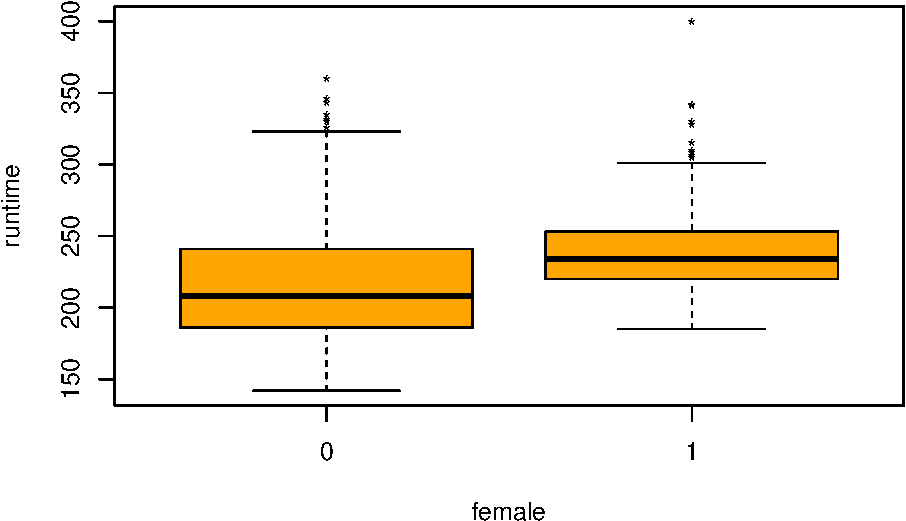
\includegraphics{HomeworkWeek4_files/figure-latex/unnamed-chunk-5-1} \end{center}

\begin{enumerate}
\def\labelenumi{\alph{enumi}.}
\setcounter{enumi}{9}
\itemsep1pt\parskip0pt\parsep0pt
\item
  Assess whether there is an interaction between female and runtime
\end{enumerate}

\begin{verbatim}
## 
## Call:
## glm(formula = nas135 ~ female * runtime, family = "binomial", 
##     data = data)
## 
## Deviance Residuals: 
##     Min       1Q   Median       3Q      Max  
## -1.1505  -0.5874  -0.3611  -0.2798   2.6786  
## 
## Coefficients:
##                 Estimate Std. Error z value Pr(>|z|)    
## (Intercept)    -6.006665   1.067610  -5.626 1.84e-08 ***
## female          1.664387   1.666037   0.999 0.317790    
## runtime         0.015392   0.004299   3.581 0.000343 ***
## female:runtime -0.002845   0.006657  -0.427 0.669123    
## ---
## Signif. codes:  0 '***' 0.001 '**' 0.01 '*' 0.05 '.' 0.1 ' ' 1
## 
## (Dispersion parameter for binomial family taken to be 1)
## 
##     Null deviance: 360.9  on 476  degrees of freedom
## Residual deviance: 324.3  on 473  degrees of freedom
##   (11 observations deleted due to missingness)
## AIC: 332.3
## 
## Number of Fisher Scoring iterations: 5
\end{verbatim}

The p-value for the interaction between female and runtime is 0.669123
and, therefore, interaction between sex and runtime is not significant
at 95\% confidence.

\begin{enumerate}
\def\labelenumi{\alph{enumi}.}
\setcounter{enumi}{10}
\itemsep1pt\parskip0pt\parsep0pt
\item
  Add to the model that contains female and runtime a dichotomous
  variable wgain which takes the value of 0 if wtidff ≤ 0, and the value
  of 1 if wtidff \textgreater{} 0. Test for interaction between female
  and wgain.
\end{enumerate}

The model including the dichotomus variable wgain described above:

\begin{verbatim}
## 
## Call:
## glm(formula = nas135 ~ female + wgain + runtime, family = "binomial", 
##     data = data2)
## 
## Deviance Residuals: 
##     Min       1Q   Median       3Q      Max  
## -1.4347  -0.4864  -0.3021  -0.1947   2.9008  
## 
## Coefficients:
##             Estimate Std. Error z value Pr(>|z|)    
## (Intercept) -7.10548    1.00104  -7.098 1.27e-12 ***
## female       0.77634    0.31667   2.452   0.0142 *  
## wgain        1.72997    0.32347   5.348 8.88e-08 ***
## runtime      0.01684    0.00380   4.431 9.38e-06 ***
## ---
## Signif. codes:  0 '***' 0.001 '**' 0.01 '*' 0.05 '.' 0.1 ' ' 1
## 
## (Dispersion parameter for binomial family taken to be 1)
## 
##     Null deviance: 337.85  on 448  degrees of freedom
## Residual deviance: 270.63  on 445  degrees of freedom
##   (39 observations deleted due to missingness)
## AIC: 278.63
## 
## Number of Fisher Scoring iterations: 6
\end{verbatim}

Including interaction between female and wgain:

\begin{verbatim}
## 
## Call:
## glm(formula = nas135 ~ female * wgain + runtime, family = "binomial", 
##     data = data2)
## 
## Deviance Residuals: 
##     Min       1Q   Median       3Q      Max  
## -1.3681  -0.5136  -0.2481  -0.1580   3.0408  
## 
## Coefficients:
##              Estimate Std. Error z value Pr(>|z|)    
## (Intercept)  -7.53350    1.06976  -7.042 1.89e-12 ***
## female        1.50083    0.52247   2.873  0.00407 ** 
## wgain         2.40100    0.51194   4.690 2.73e-06 ***
## runtime       0.01688    0.00389   4.340 1.43e-05 ***
## female:wgain -1.20186    0.66094  -1.818  0.06900 .  
## ---
## Signif. codes:  0 '***' 0.001 '**' 0.01 '*' 0.05 '.' 0.1 ' ' 1
## 
## (Dispersion parameter for binomial family taken to be 1)
## 
##     Null deviance: 337.85  on 448  degrees of freedom
## Residual deviance: 267.22  on 444  degrees of freedom
##   (39 observations deleted due to missingness)
## AIC: 277.22
## 
## Number of Fisher Scoring iterations: 6
\end{verbatim}

The interaction is not significant at 95\% but it is at 90\% confidence.

\begin{enumerate}
\def\labelenumi{\alph{enumi}.}
\setcounter{enumi}{11}
\itemsep1pt\parskip0pt\parsep0pt
\item
  On the basis of the model with the interaction term, calculate the
  Odds Ratios of hyponatremia for males who gain weight as compared to
  those who don't. Repeat this exercise for a female. Interpret your
  findings.
\end{enumerate}

For males, the odd ratio of those who gain weigth vs.~those who doesn't
is $e^{2.40100}$ = 11.0342069\\For females, the odd ratio of those who
gain weigth vs.~those who doesn't is $e^{2.40100-1.20186}$ = 3.3172774

A male who experiences weight gain during a marathon has an odds of
hyponatremia 11.0342069 times higher than that of a male who does not
gain weight. On the other hand, a female who experiences weight gain
during a marathon has an odds of hyponatremia 3.3172774 times higher
than that of a female who does not gain weight.

\begin{enumerate}
\def\labelenumi{\alph{enumi}.}
\setcounter{enumi}{12}
\itemsep1pt\parskip0pt\parsep0pt
\item
  Compare using the Likelihood Ratio test the model with female and
  runtime with a model with female, runtime, wgain, urinat3p and bmi.
  (Hint: the 2 models must be fitted on the same set of observations. Be
  aware of missing values in some of these variables). How many degrees
  of freedom does the test statistic have?
\end{enumerate}

We exclude all missing values and run the model with all variables

\begin{verbatim}
## 
## Call:
## glm(formula = nas135 ~ female + wgain + runtime + urinat3p + 
##     bmi, family = "binomial", data = data3)
## 
## Deviance Residuals: 
##     Min       1Q   Median       3Q      Max  
## -1.4099  -0.4711  -0.2969  -0.2000   2.8722  
## 
## Coefficients:
##              Estimate Std. Error z value Pr(>|z|)    
## (Intercept) -6.565610   1.599794  -4.104 4.06e-05 ***
## female       0.759657   0.415521   1.828  0.06752 .  
## wgain        1.735328   0.330983   5.243 1.58e-07 ***
## runtime      0.014701   0.004839   3.038  0.00238 ** 
## urinat3p     0.815514   0.551410   1.479  0.13915    
## bmi         -0.004152   0.074235  -0.056  0.95540    
## ---
## Signif. codes:  0 '***' 0.001 '**' 0.01 '*' 0.05 '.' 0.1 ' ' 1
## 
## (Dispersion parameter for binomial family taken to be 1)
## 
##     Null deviance: 328.17  on 441  degrees of freedom
## Residual deviance: 263.23  on 436  degrees of freedom
## AIC: 275.23
## 
## Number of Fisher Scoring iterations: 6
\end{verbatim}

On the dataset with no missing values we run the model with female and
runtime variables only:

\begin{verbatim}
## 
## Call:
## glm(formula = nas135 ~ female + runtime, family = "binomial", 
##     data = data3)
## 
## Deviance Residuals: 
##     Min       1Q   Median       3Q      Max  
## -1.2198  -0.5626  -0.3677  -0.2880   2.6724  
## 
## Coefficients:
##              Estimate Std. Error z value Pr(>|z|)    
## (Intercept) -5.959965   0.897346  -6.642 3.10e-11 ***
## female       0.873966   0.305045   2.865  0.00417 ** 
## runtime      0.015205   0.003589   4.236 2.27e-05 ***
## ---
## Signif. codes:  0 '***' 0.001 '**' 0.01 '*' 0.05 '.' 0.1 ' ' 1
## 
## (Dispersion parameter for binomial family taken to be 1)
## 
##     Null deviance: 328.17  on 441  degrees of freedom
## Residual deviance: 296.48  on 439  degrees of freedom
## AIC: 302.48
## 
## Number of Fisher Scoring iterations: 5
\end{verbatim}

The p-value of the likelihood test (based on the deviance of both models
provided by R) is 2.8557397\times 10\^{}\{-7\} so we can confirm that
the model with 5 variables is better than the one with only 2.

A model including only female, runtime and wgain:

\begin{verbatim}
## 
## Call:
## glm(formula = nas135 ~ female + runtime + wgain, family = "binomial", 
##     data = data3)
## 
## Deviance Residuals: 
##     Min       1Q   Median       3Q      Max  
## -1.4070  -0.4798  -0.2996  -0.1988   2.8840  
## 
## Coefficients:
##              Estimate Std. Error z value Pr(>|z|)    
## (Intercept) -6.973049   1.013843  -6.878 6.08e-12 ***
## female       0.700105   0.320203   2.186   0.0288 *  
## runtime      0.016359   0.003879   4.217 2.48e-05 ***
## wgain        1.759529   0.328242   5.360 8.30e-08 ***
## ---
## Signif. codes:  0 '***' 0.001 '**' 0.01 '*' 0.05 '.' 0.1 ' ' 1
## 
## (Dispersion parameter for binomial family taken to be 1)
## 
##     Null deviance: 328.17  on 441  degrees of freedom
## Residual deviance: 265.36  on 438  degrees of freedom
## AIC: 273.36
## 
## Number of Fisher Scoring iterations: 6
\end{verbatim}

Now, the p-value of the likelihood test comparing the model with all
variables and the one with three is 0.3460079 so we can confirm that the
model without bmi and urine variables is better.

\end{document}
